% arara: pdflatex
\documentclass{beamer}
\usepackage[utf8]{inputenc}

\title{\Huge\texttt{vim} \\ \normalsize ``Who needs a mouse?''}
\author{Nicolas Dorrmann}
\date{04. Nov. 2020}

\begin{document}

\frame{\titlepage}

\begin{frame}
    \frametitle{History and Design Philosophy}
    \begin{itemize}
        \item Developed by Bram Moolenaar, initially released in 1991.
        \item Successor to \texttt{vi} (\textbf{v}isual \textbf{i}nterface for line editor \texttt{ex}).
        \item Editing works entirely over keyboard, most commands are easily reachable over home row.
        \item Plugins (written in \texttt{VimScript}) \textit{can} provide functionality similar to an IDE.
    \end{itemize}
\end{frame}
\begin{frame}
    \frametitle{But why?}
    \begin{itemize}
        \item It's everywhere (if you want it) --- a lot of software has the option of using \texttt{vim} keybindings.
        \begin{description}
            \item [\texttt{qutebrowser}]  webbrowser
            \item [\texttt{vifm}]         filemanager
            \item [\texttt{IdeaVim}]      \texttt{vim} keybindings for JetBrains IDEs
            \item [\texttt{ExcelLikeVim}] \texttt{vim} keybindings for MS Excel (yes, seriously)
        \end{description}
        \item It's versatile --- lightweight text editor or almost-universal IDE (or anything in between).
        \item It's ``intuitive'' --- after getting used to it, you can use \texttt{vim} almost like a language.
    \end{itemize}
\end{frame}
\begin{frame}
    \frametitle{Basics}
    \begin{itemize}
        \item Modes
            \begin{description}
                \item [\texttt{NORMAL}]  navigate within the file, issue text commands (yank/change/delete)
                \item [\texttt{COMMAND}] open, close, or save a file
                \item [\texttt{INSERT}]  direct input (i.\ e.\ actually typing text)
                \item [\texttt{VISUAL}]  text highlighting, text blocking
            \end{description}
    \end{itemize}
    \vspace{0.5cm}
    \begin{center}
        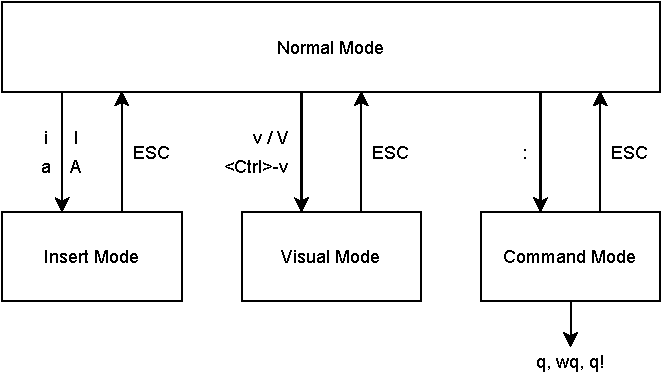
\includegraphics[width=0.6\textwidth]{graphics/vim_modes.pdf}
    \end{center}
\end{frame}
\begin{frame}
    \frametitle{Basics}
    \begin{itemize}
        \item Actions (``verbs'')
            \begin{description}
                \item [\textbf{y}ank]   copy a movement
                \item [\textbf{c}hange] replace object with a new object
                \item [\textbf{d}elete] remove an object
            \end{description}
        \item Modifiers
            \begin{description}
                \item [\texttt{NUM}] number of objects to perform action on
                \item [\texttt{i}]   perform action \textbf{i}nside an object
                \item [\texttt{a}]   perform action \textbf{a}round an object
                \item [\texttt{t}]   perform action up \textbf{t}o an object
                \item [\texttt{f}]   perform action up to and including an object
            \end{description}
        \item Text Objects (``nouns'')
            \begin{description}
                \item [\textbf{w}ord]      string of non-whitespace characters surrounded by whitespace
                \item [\textbf{s}entence]  ends with \texttt{!}, \texttt{?}, \texttt{.} followed by newline
                \item [\textbf{p}aragraph] consists of several sentences, delimited by empty lines
            \end{description}
    \end{itemize}
\end{frame}
\begin{frame}
    \frametitle{Commands}
    \begin{itemize}
        \item Commands have the form \texttt{Action} --- \texttt{Modifier} --- \texttt{Object}
        \item Examples
        \begin{description}
            \item [\texttt{y2w}] copy the next two words
            \item [\texttt{dis}] delete the current sentence (i.\ e.\ the sentence the cursor is in)
            \item [\texttt{cp}]  change (i.\ e.\ delete and enter \texttt{INSERT} mode) the current paragraph
        \end{description}
    \end{itemize}
\end{frame}

\end{document}

